\Section{Experimental Setup}

In this chapter the experimental context of this thesis will be discussed. 

\Subsection{The Large Hadron Collider}
\label{sec:theory}

The Large Hadron Collider (LHC) is currently the most powerful particle accelerator in the world. Hosted at CERN in Geneva at the Swiss-French border and first put into operation on $\text{10}^\text{th}$ September 2008, the LHC is designed for proton and heavy lead ion collisions. The machine has gone through several upgrades between the consecutive data-taking phases (Runs) called Long Shutdowns (LS). During these the proton beam energy has been gradually increased from \SI{3.5}{\tera\electronvolt} to a recently -- on the $\text{5}^{\text{th}}$ July, 2022 to be precise -- achieved energy of \SI{6.8}{\tera\electronvolt} \cite{Alici:2773265} resulting in a total centre-of-mass (CM) proton-proton collision energy of $\sqrt{s} = \SI{13.6}{\tera\electronvolt}$. Similarly, the beam intensity has seen an increase from $1.1 \times 10^{11}$ protons per bunch (ppb) and \textasciitilde200 bunches to a projected \textasciitilde$1.8 \times 10^{11}$ ppb and \textasciitilde2500 bunches \cite{Fartoukh:2790409, Karastathis:2750302}. With a theoretical maximum CM energy of $\sqrt{s} = \SI{14}{\tera\electronvolt}$ and integrated luminosity of $L = \SI{10d34}{\centi\meter^{-2}\second^{-1}}$ it holds the record in these measures among concurring experiments. In order to achieve such luminosities, the beams are kept on a circular trajectory using superconducting NbTi magnets operating at \SI{1.9}{\kelvin} thanks to the superfluid helium bath at about \SI{0.13}{\mega\pascal} \cite{Brüning:782076}.

As a result of consecutive accelerator upgrades, the collider complex has an impressive and complex pre-accelerator structure as shown in fig. \ref{fig:lhcstructure}. Consequently, the proton bunches first go through multiple preparation steps before they get injected into the \SI{27}{\kilo\meter} tunnel of the LHC where the four main experiments (ALICE, ATLAS, LHCb and CMS) and their interaction points are located. 

\begin{figure}[h!]
	\centering
	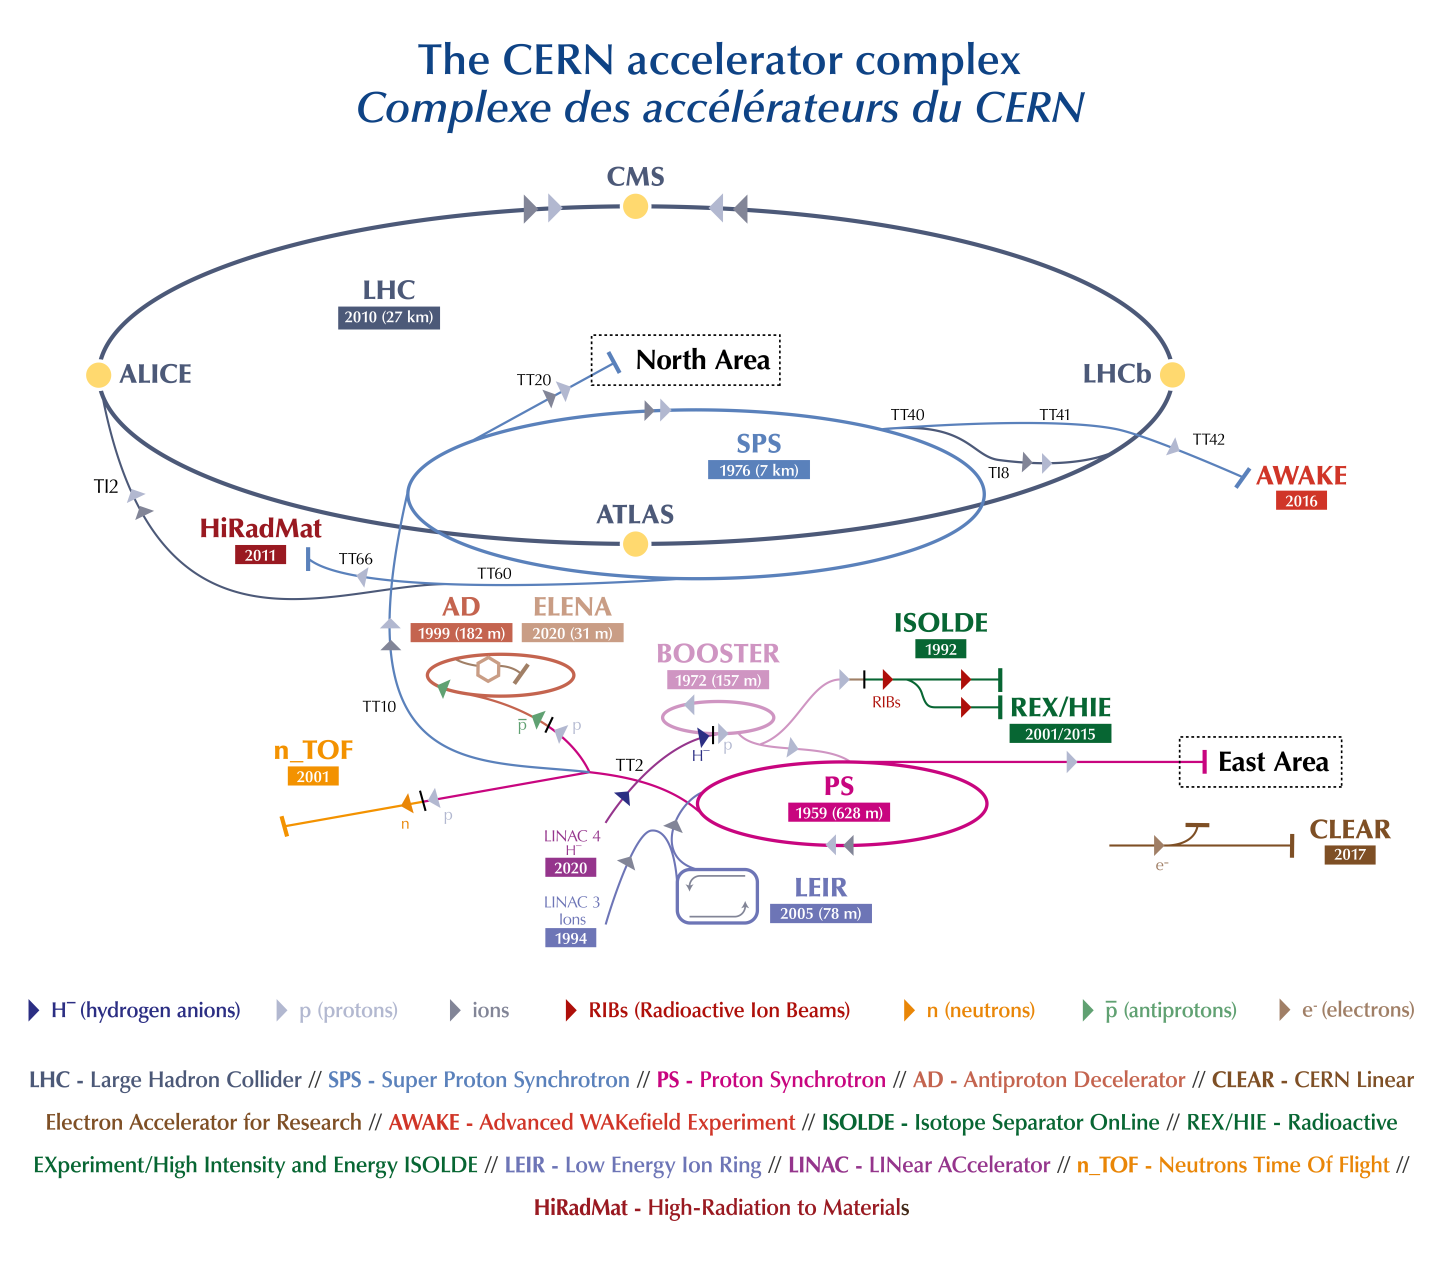
\includegraphics[width=\textwidth]{figures/theoryexperiment/CCC-v2019-final-white}
	\caption{The accelerator complex of the LHC, their corresponding construction years and circumferences. Individual stages are shown in different colours, the particle types they accelerate are indicated as arrows. Note that the pre-acceleators do not serve the LHC ring exclusively and the diverging paths lead to other independent experiments. Old tunnels of previous experiments serve as pre-accelerators now in the LHC injection chain. \cite{Mobs:2684277}}
	\label{fig:lhcstructure}
\end{figure}

The four main stages of pre-acceleration for protons are listed in \ref{tab:preaccelerators} below. As proton source, hydrogen is used. The protons are first accelerated in the form of H$^-$ ions through the 86 metre long tunnel of the recently (2020) constructed Linear Accelerator 4 (Linac4). Stripped of their pair of electrons, the protons enter the Proton Synchrotron Booster (PSB) where they reach up to \SI{2}{\giga\electronvolt}. In the next step of the injection chain, they enter the Proton Synchrotron (PS), historically the first synchrotron at CERN serving exclusively as a pre-accelerator now. Travelling through the 628 metres long ring and accelerated to 26 GeV, the particles are injected into the Super Proton Synchrotron (SPS), where they are awaiting injection into the LHC once they reach 450 GeV.

\begin{table}[h!]
	\centering
	\begin{tabular}{c|c}
		Accelerator & Peak Energy \\
		\hline
		\hline
		Linear accelerator 4 (Linac4) & 160 MeV \\
		\hline
		Proton Synchrotron Booster (PSB) & 2 GeV \\
		\hline
		Proton Synchrotron (PS) & 26 GeV \\
		\hline
		Super Proton Synchrotron (SPS) & 450 GeV \\
		\hline
		Large Hadron Collider (LHC) & 7 TeV \\
	\end{tabular}
	\caption{The acceleration chain the protons undergo to reach their final energy of 7 TeV.}
	\label{tab:preaccelerators}
\end{table}

\color{red}{Entering the LHC, they live happily forever after until they are brutally crushed into each other and die of quantum mechanics.}\color{black}



\Subsection{The Compact Muon Solenoid}

One of general purpose detectors at the Large Hadron Collider at CERN is the Compact Muon Solenoid (CMS).
